\chapter{Giới thiệu tổng quan đề tài}
Chương này sẽ giới thiệu về một trong những vấn đề thách thức trong vận hành mạng lưới viễn thông đó là quản lí thiết bị viễn thông. Và tái tạo mô hình đám mây điểm 3D chi tiết, chính xác là một trong những bài toán đặc biệt quan trọng. Trong đó, đảm bảo tính chính xác trong việc tính toán camera pose trở thành yếu tố then chốt quyết định trực tiếp tới chất lượng của mô hình.

\section{Lí do chọn đề tài và tính cấp thiết}
Trong kỷ nguyên số hóa và sự bùng nổ của công nghệ viễn thông, đặc biệt là mạng 5G và các thế hệ tiếp theo, hạ tầng mạng lưới viễn thông ngày càng trở nên phức tạp và quy mô hơn bao giờ hết. Theo số liệu đầu năm 2019 \cite{viettel_construction_2020} thì tổng số lượng cột ăng-ten của ba nhà mạng lớn tại Việt Nam gồm: Viettel, Vinaphone, Mobifone đạt khoảng 100000 cột. Việc quản lý hiệu quả hàng trăm nghìn cột và hàng triệu thiết bị vô tuyến gắn trên các cột ăng-ten này là một thách thức lớn đối với các nhà mạng. Phương pháp quản lý, kiểm kê, bảo trì trạm được các nhà mạng áp dụng chủ yếu hiện nay là thuê nhân công trèo lên các cột ăng-ten để đo đạc các thông số cột, thông số thiết bị, kiểm tra dấu hiệu lỗi, hỏng hóc và chụp ảnh bằng điện thoại, sau đó gửi lại thông tin cho người quản lí trạm. Phương án khảo sát cột thủ công này không chỉ tốn kém về chi phí nhân công, thời gian mà còn tiềm ẩn nhiều sai sót, khó đáp ứng được yêu cầu về độ chính xác trong vận hành và tối ưu hóa mạng lưới. 

Trong bối cảnh đó, số hóa trạm viễn thông là giải pháp tất yếu mà các nhà mạng lớn cần thực hiện. Giải pháp này không chỉ giảm chi phí vận hành mà còn nâng cao độ chính xác khi khảo sát các thông tin kỹ thuật của cột và thiết bị trên cột. Để thực hiện tốt giải pháp số hóa trạm viễn thông, xây dựng mô hình đám mây điểm 3D chi tiết, chính xác của cột ăng-ten như mô tả trong Hình \ref{fig:gen-3d-pc} là một trong những bài toán quan trọng nhất. Đây là quá trình sử dụng các thuật toán xử lý hình học hoặc học sâu để chuyển hóa thông tin ảnh chụp 2D đa góc nhìn xung quanh cột thành một mô hình đám mây điểm 3D dày đặc, chính xác. Việc xây dựng một mô hình đám mây điểm 3D tốt là điều kiện tiên quyết thực hiện các bài toán như: tự động hóa tính toán các thông số kỹ thuật của cột và thiết bị trên cột, cũng như các bài toán mô phỏng vùng phủ sóng của cột.

\begin{figure}
    \centering
    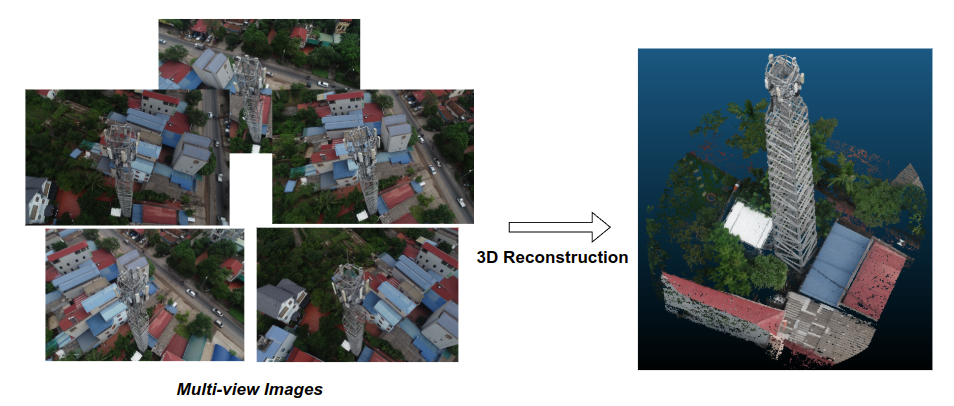
\includegraphics[width=0.8\linewidth]{figures/c1/gen_3d_pc.png}
    \caption{Minh họa chuyển đổi các bức ảnh 2D đa góc nhìn thành mô hình mây điểm 3D chi tiết.}
    \label{fig:gen-3d-pc}
\end{figure}

Điều kiện tiên quyết để tạo ra được một mô hình đám mây điểm 3D chi tiết, chất lượng cao đó là ước tính chính xác camera pose cho các bức ảnh 2D chụp xung quanh cột ăng-ten. Trong đó, camera pose là thông tin đầu vào quan trọng cho bước tái tạo mô hình 3D, thể hiện vị trí và hướng của máy ảnh trong hệ tọa độ thế giới, được biểu diễn bằng 6 bậc tự do (6DoF): 3 bậc tự do cho dịch chuyển $(x, y, z)$ và 3 bậc tự do quay $(pitch, yaw, roll)$. Camera pose thường được biểu diễn bằng ma trận biến đổi hoặc cặp $(R, t)$, trong đó $R$ là ma trận quay và $t$ là véc-tơ dịch chuyển \cite{xu2022critical}. Nó quyết định trực tiếp tới độ chính xác của các điểm 3D được tái tạo. Tuy nhiên việc ước tính camera pose trong thực tế gặp rất nhiều thách thức. Nguyên nhân là bởi cột ăng-ten của trạm viễn thông có kiến trúc lặp, cấu tạo bởi nhiều thành phần kim loại và hệ thống cáp phức tạp. Nhưng xét trên phương diện tái tạo 3D từ hình ảnh, một đặc điểm nổi bật và gây nhiều thách thức nhất cho các thuật toán chính là bề mặt của các thiết bị vô tuyến được lắp đặt trên cột. Cụ thể, bề mặt các thiết bị như ăng-ten, RRU làm từ nhựa hoặc composite, lớp vỏ này có bề mặt rất trơn nhẵn, đồng nhất về màu sắc (thường là trắng hoặc xám nhạt) và hầu như không có họa tiết hay các điểm đặc trưng trực quan rõ ràng. Đặc tính thiếu đặc trưng bề mặt này làm cho việc đối sánh điểm ảnh giữa các góc nhìn khác nhau trở nên cực kỳ khó khăn, dẫn đến sai số lớn hoặc thất bại trong giai đoạn ước tính camera pose.

Sau khi tính toán thông tin camera pose từ giai đoạn đầu, các phương pháp tái tạo dày đặc như Tái tạo lập thể đa góc nhìn (MVS) hoặc các kỹ thuật mới hơn dựa trên học sâu như Trường bức xạ nơ-ron (NeRF) thường được sử dụng để tạo ra mô hình đám mây điểm 3D chi tiết cuối cùng. Do vậy, chất lượng của mô hình tái tạo phụ thuộc rất lớn vào độ chính xác của camera pose đầu vào. Nếu camera pose của các bức ảnh có sai số lớn thì mô hình mây điểm 3D sẽ chứa nhiều điểm nhiễu và không đảm bảo cấu trúc hình học.

Xuất phát từ những phân tích về tính khả thi và cấp thiết của bài toán xây dựng mô hình đám mây điểm 3D chi tiết, chính xác đối với vấn đề quản lí thiết bị vô tuyến, đề tài "Nghiên cứu các mô hình học sâu cho bài toán quản lí thiết bị vô tuyến" được thực hiện với mục tiêu đề xuất một giải pháp cải tiến, hiệu quả nhằm nâng cao độ chính xác khi tính toán camera pose cho các bức ảnh chụp 2D đầu vào, nhằm xây dựng mô hình 3D chi tiết, chất lượng cao cho đối tượng cột ăng-ten của trạm viễn thông. Luận văn sẽ đi sâu vào nghiên cứu, thử nghiệm các kỹ thuật cải tiến so với phương pháp truyền thống, và thực hiện đánh giá, so sánh độ hiệu quả của các phương pháp trên các tập dữ liệu trạm viễn thông thực tế. Bên cạnh đó, luận văn cũng đưa ra những phân tích, so sánh, đánh giá ưu, nhược điểm của các giải pháp tái tạo đám mây điểm 3D truyền thống và hiện đại khi áp dụng vào bài toán thực tế cho đối tượng cột ăng-ten. Từ đó, mở ra tiềm năng ứng dụng giải pháp vào thực tiễn cho các nhà mạng viễn thông trong và ngoài nước.

% Các phương pháp tái tạo 3D truyền thống dựa trên hình ảnh, như thuật toán Tái tạo lập thể đa góc nhìn (MVS), đã được nghiên cứu và ứng dụng vào các bài toán khác nhau trong nhiều năm. Đây là một phương pháp tiêu chuẩn với nhiều điểm mạnh khi xây dựng mô hình đám mây điểm 3D, đặc biệt là đảm bảo độ chính xác cao về cấu trúc hình học. Bên cạnh đó, với sự phát triển của các mô hình học sâu, các phương pháp mới ứng dụng mạng học sâu cho thuật toán MVS ra đời như MVSNet, MVSNet++, HighRes-MVSNet,... cho thấy những kết quả đầy hứa hẹn khi áp dụng vào các bài toán thực tế. Một hướng tiếp cận hiện đại và tiềm năng khác, đó là sự xuất hiện của mô hình Trường bức xạ nơ-ron (NeRF). NeRF sử dụng sức mạnh của mạng nơ-ron sâu để học trực tiếp một biểu diễn liên tục, ẩn của trường bức xạ 5D (màu sắc và mật độ thể tích tại mọi điểm 3D theo mọi hướng nhìn). Ưu điểm cốt lõi của NeRF là khả năng xử lý các bề mặt khó (như bề mặt trơn, bóng) tốt hơn so với MVS do cơ chế học dựa trên tối ưu hóa hàm lỗi quang học trên toàn bộ tia nhìn thay vì chỉ dựa vào đối sánh đặc trưng cục bộ. Nhưng trên tất cả, chất lượng của mô hình đám mây điểm 3D được tái tạo từ các phương pháp kể trên phụ thuộc rất lớn vào độ chính xác của camera pose đầu vào.

% Các phương pháp tái tạo 3D truyền thống dựa trên hình ảnh, như Phục dựng cấu trúc từ chuyển động (SfM) kết hợp với thuật toán Tái tạo lập thể đa góc nhìn (MVS), đã được nghiên cứu và ứng dụng vào các bài toán khác nhau trong nhiều năm. Tuy nhiên, các phương pháp này lại bộc lộ những hạn chế đáng kể khi áp dụng vào bài toán cụ thể này. Quy trình SfM kết hợp MVS có thể đòi hỏi thời gian xử lý lớn, đặc biệt với số lượng ảnh lớn, độ phân giải cao. Quan trọng hơn, chất lượng tái tạo của MVS phụ thuộc nhiều vào sự hiện diện của các đặc trưng bề mặt phong phú; do đó, chúng thường gặp khó khăn và cho kết quả thiếu chi tiết, nhiễu hoặc thậm chí thất bại khi xử lý các đối tượng có bề mặt ít hoặc không có họa tiết, bề mặt trơn nhẵn, hoặc có tính phản xạ cao - vốn là đặc điểm phổ biến của các thiết bị như ăng-ten hay RRU. Kết quả là mô hình đám mây điểm 3D cột ăng-ten thu được từ các phương pháp truyền thống thường không đủ độ chi tiết, thủng rỗng bề mặt các thiết bị.

% Trong bối cảnh đó, sự ra đời và phát triển nhanh chóng của mô hình Trường bức xạ nơ-ron (NeRF) và các biến thể của nó đã mở ra một hướng tiếp cận mới đầy tiềm năng. NeRF sử dụng sức mạnh của mạng nơ-ron sâu để học trực tiếp một biểu diễn liên tục, ẩn của trường bức xạ 5D (màu sắc và mật độ thể tích tại mọi điểm 3D theo mọi hướng nhìn) từ một tập hợp các ảnh 2D và thông tin vị trí, hướng của máy ảnh khi chụp mỗi bức ảnh tương ứng. Thông qua kỹ thuật kết xuất thể tích, NeRF có khả năng tổng hợp hình ảnh tại các góc nhìn mới với chất lượng chân thực và độ chi tiết ấn tượng, ngay cả đối với các cấu trúc, bối cảnh phức tạp. Ưu điểm cốt lõi của NeRF là khả năng xử lý các bề mặt khó (như bề mặt trơn, bóng) tốt hơn so với MVS do cơ chế học dựa trên tối ưu hóa hàm lỗi quang học trên toàn bộ tia nhìn thay vì chỉ dựa vào đối sánh đặc trưng cục bộ. Trong những năm gần đây, cộng đồng nghiên cứu về NeRF đang phát triển rất nhanh, liên tục đề xuất các biến thể NeRF mới giúp cải thiện đáng kể tốc độ huấn luyện, giảm yêu cầu tài nguyên tính toán, tăng cường độ phân giải và đặc biệt là nâng cao độ chính xác cấu trúc hình học khi tái tạo mô hình 3D so với phiên bản NeRF gốc. Những ưu điểm này làm cho NeRF trở thành một công nghệ tiềm năng cho bài toán xây dựng mô hình 3D chi tiết, chất lượng cao cho cột ăng-ten của các trạm viễn thông.

% Mặc dù sở hữu nhiều ưu điểm vượt trội, việc áp dụng trực tiếp các mô hình NeRF tiêu chuẩn vào nhiệm vụ đòi hỏi độ chính xác hình học cao như xây dựng mô hình 3D cho cột ăng-ten của bài toán quản lý cột và thiết bị viễn thông vẫn còn những thách thức và hạn chế. Cơ chế và bản chất cốt lõi của NeRF là tập trung vào việc nâng cao khả năng kết xuất hình ảnh thông qua việc huấn luyện mạng học sâu học biểu diễn ẩn một không gian 5D (gồm vị trí và màu sắc). Việc này dẫn đến những bất ổn hoặc sai lệch về mặt cấu trúc hình học tuyệt đối khi tái tạo mô hình 3D từ biểu diễn ẩn này. Xuất phát từ những phân tích về tiềm năng của NeRF cũng như những yêu cầu thực tiễn của ngành viễn thông, đề tài "Nghiên cứu các mô hình học sâu cho bài toán quản lí thiết bị vô tuyến" được thực hiện với mục tiêu đề xuất một giải pháp tiên tiến, hiệu quả dựa trên nền tảng NeRF, nhằm xây dựng mô hình 3D chi tiết, chất lượng cao, và đặc biệt là đảm bảo độ chính xác về cấu trúc hình học cho đối tượng cột ăng-ten của trạm viễn thông. Luận văn sẽ đi sâu vào nghiên cứu, thử nghiệm các mô hình biến thể cải thiện độ chính xác cấu trúc hình học của NeRF với các tập dữ liệu chuẩn như DTU, Tanks and Temples và các tập dữ liệu hình ảnh thực tế của các trạm viễn thông; sau đó, luận văn đưa ra những phân tích, so sánh, đánh giá ưu nhược điểm của từng mô hình. Từ đó, mở ra tiềm năng ứng dụng giải pháp vào thực tế cho các nhà mạng viễn thông trong và ngoài nước.

\section{Mục tiêu nghiên cứu}
Luận văn hướng tới việc nghiên cứu, đề xuất kỹ thuật cải thiện độ chính xác tính toán camera pose trong việc xây dựng mô hình 3D chi tiết, chất lượng cao cho đối tượng cột ăng-ten của trạm viễn thông, đáp ứng tốt các yêu cầu của bài toán quản lý thiết bị vô tuyến trong thực tế. Các mục tiêu nghiên cứu chính bao gồm:
\begin{itemize}
    \item Xác định và phân tích hạn chế: Đánh giá và làm rõ được những hạn chế của các phương pháp tính toán camera pose phổ biến hiện nay khi áp dụng cho dữ liệu ảnh chụp 2D cột ăng-ten của trạm viễn thông trong điều kiện thực tế.

    \item Trình bày các phân tích, so sánh, đánh giá chi tiết giữa các giải pháp tái tạo mô hình 3D truyền thống MVS và các giải pháp dựa trên học sâu như NeRF khi ứng dụng cho bài toán tái tạo đám mây điểm 3D chi tiết, chính xác cho đối tượng cột ăng-ten. Từ đó, đưa ra giải pháp tối ưu cho bài toán thực tế này.
    
\end{itemize}
 
Bên cạnh đó, luận văn còn hướng tới việc đóng góp một giải pháp kỹ thuật có tiềm năng ứng dụng cao, giải quyết một nhu cầu cấp thiết trong ngành viễn thông, đồng thời thúc đẩy nghiên cứu ứng dụng học sâu và thị giác máy tính tại Việt Nam.

\section{Đối tượng và phạm vi nghiên cứu}
Đối tượng nghiên cứu chính của luận văn này tập trung vào các kỹ thuật trích xuất, khớp nối đặc trưng truyền thống và các kỹ thuật trích xuất, khớp nối dựa trên học sâu. Luận văn cũng nghiên cứu về các thuật toán tái tạo đám mây điểm 3D từ ảnh 2D và camera pose tương ứng, và đánh giá trong bối cảnh cụ thể là tái tạo mô hình đám mây điểm 3D cho cột ăng-ten của các trạm viễn thông Do đó, các đặc điểm của cột ăng-ten (cấu trúc phức tạp, khoảng cách chụp xa, kích thước lớn, môi trường ngoài trời) và dữ liệu ảnh (chất lượng, số lượng, góc chụp) cũng là những yếu tố được xem xét trong phạm vi đối tượng nghiên cứu của luận văn khi đánh giá hiệu quả của các phương pháp.

\section{Phương pháp nghiên cứu}
Phương pháp nghiên cứu của luận văn là sự kết hợp giữa nghiên cứu lý thuyết và nghiên cứu thực nghiệm. Quá trình nghiên cứu được tiến hành qua các giai đoạn chính sau:
\begin{itemize}
    \item  Nghiên cứu tổng quan và nghiên cứu sâu các kiến thức nền tảng về luồng thực hiện tái tạo 3D từ ảnh 2D: SfM, MVS, và các phương pháp dựa trên NeRF.
    \item Nghiên cứu các thuật toán phát hiện, mô tả và khớp nối đặc trưng: truyền thống (SIFT) và dựa trên học sâu (ALIKED, LightGlue).
    \item Nghiên cứu các phương pháp và chỉ số để đánh giá độ chính xác của camera pose và chất lượng của mô hình 3D tái tạo.
    \item Thử nghiệm và kiểm chứng tính hiệu quả: 
    \begin{itemize}
        \item Thực hiện các thử nghiệm nhằm kiểm tra tính hiệu quả của các phương pháp cải thiện độ chính xác tính toán camera pose đề xuất.
        \item Phân tích so sánh chất lượng tái tạo mô hình mây điểm 3D của các phương pháp truyền thống MVS và phương pháp hiện đại dựa trên NeRF, với đầu vào là camera pose của phương pháp đề xuất và camera pose của phương pháp truyền thống.
    \end{itemize}
   
\end{itemize}

\section{Đóng góp chính của luận văn}
    Các đóng góp nghiên cứu khoa học chính của luận văn:
    \begin{itemize}
        \item Đề xuất giải pháp, được gọi là Hybrid-SfM nhằm cải thiện độ chính xác tính toán camera pose để tạo đầu vào tốt nhất cho giai đoạn tái tạo chi tiết đám mây điểm 3D. Thử nghiệm, đánh giá độ hiệu quả của phương pháp đề xuất với 5 bộ dữ liệu ảnh chụp đối tượng cột ăng-ten, trạm viễn thông thực tế.
        \item Nghiên cứu, thử nghiệm, đánh giá độ hiệu quả của các công nghệ tái tạo đám mây điểm 3D chi tiết, dày đặc truyền thống như MVS và hiện đại như NeRF trong việc tái tạo đám mây điểm 3D chi tiết, chính xác cho đối tượng cột ăng-ten với 5 bộ dữ liệu trạm viễn thông thực tế.  Đánh giá tiềm năng ứng dụng thực tiễn của giải pháp cho các nhà mạng viễn thông tại Việt Nam.
    \end{itemize}
\section{Bố cục luận văn}
Ngoài phần Tóm tắt, Danh mục tài liệu tham khảo, nội dung chính của luận văn được tổ chức thành 5 chương như sau:
\begin{itemize}
    \item Chương 1: Giới thiệu tổng quan đề tài. Chương này trình bày lý do chọn đề tài, tính cấp thiết của đề tài trong việc nghiên cứu các mô hình học sâu giải quyết bài toán tái tạo mô hình 3D chính xác cho vấn đề quản lý hạ tầng viễn thông. Đồng thời, chương xác định rõ mục tiêu nghiên cứu, đối tượng, phạm vi nghiên cứu, phương pháp nghiên cứu và những đóng góp nghiên cứu khoa học chính của luận văn. Đồng thời trình bày bố cục tổng thể của các chương tiếp theo.

    \item Chương 2: Cơ sở lý thuyết. Chương này cung cấp nền tảng kiến thức lý thuyết cần thiết cho luận văn. Nội dung bao gồm giới thiệu về bài toán tái tạo đám mây điểm 3D và chi tiết, cách tiếp cận ước tính camera pose của thuật toán SfM truyền thống và các thuật toán trích xuất đặc trưng hiện đại. Bên cạnh đó, chương này cũng giới thiệu các phương pháp tái tạo đám mây điểm 3D chi tiết, dày đặc phổ biến: MVS và NeRF.

    \item Chương 3: Phương pháp đề xuất. Chương này tập trung trình bày chi tiết kỹ thuật đề xuất Hybrid-SfM nhằm nâng cao độ chính xác khi tính toán camera pose cho dữ liệu ảnh cột ăng-ten, trạm viễn thông. 
    
    \item Chương 4: Thực nghiệm và thảo luận. Chương này trình bày quá trình thiết lập và tiến hành các thực nghiệm nhằm kiểm chứng và đánh giá hiệu quả của kỹ thuật đề xuất. Nội dung bao gồm mô tả chi tiết về các bộ dữ liệu được sử dụng, các độ đo đánh giá, môi trường cài đặt và các kịch bản thực nghiệm. Các kết quả định lượng và định tính thu được sẽ được trình bày, so sánh giữa các phương pháp với nhau. Cuối chương là phần thảo luận, phân tích sâu về kết quả, chỉ ra ưu nhược điểm của phương pháp đề xuất khi áp dụng vào bài toán thực tế là tái tạo mô hình đám mây điểm 3D chất lượng cao cho cột ăng-ten của trạm viễn thông.
    
    \item Chương 5: Kết luận. Phần cuối cùng tóm tắt lại những kết quả chính và đóng góp cốt lõi của luận văn. Đồng thời, chương cũng chỉ ra những hạn chế còn tồn tại của nghiên cứu và đề xuất các hướng phát triển, cải tiến tiềm năng trong tương lai.
\end{itemize}



\section*{Kết luận Chương 1}
\addcontentsline{toc}{section}{Kết luận Chương 1}
Trong chương này, vấn đề quản lý thiết bị viễn thông và đặc biệt là bài toán tái tạo đám mây điểm 3D chi tiết, dày đặc đã được giới thiệu một cách tổng quan. Bên cạnh đó, mục tiêu, hướng nghiên cứu cũng như phương pháp nghiên cứu của đề tài cũng được trình bày một cách rõ ràng. Chương tiếp theo sẽ trình bày những kiến thức nền tảng về các thuật toán, kĩ thuật và các vấn đề trong tái tạo đám mây điểm 3D chi tiết, dày đặc từ tập các ảnh 2D.